\documentclass{article}
\usepackage{graphicx} 
\usepackage{hyperref}
\usepackage{subcaption}
\usepackage{amsmath}
\usepackage[colorinlistoftodos]{todonotes}

\title{Leveraging Knowledge Graphs for dimensionality reduction and interpretablity in biomedical datasets}
\author{First Author, Second Author, Third Author}
\date{July 2025}

\begin{document}

\maketitle

\section{Introduction} 
% High dimensionality of biomedical datasets
Modern biomedical research increasingly relies on high-throughput technologies, such as genomics, proteomics, and transcriptomics, which generate datasets characterized by an unprecedented number of variables. This surge in data dimensionality, moving beyond the constraints of traditional low-dimensional analyses, presents a complex array of analytical challenges . These datasets are not only vast in terms of the number of features but also inherently intricate, often domain-specific, and necessitate significant effort in feature engineering. The "curse of dimensionality" poses a significant obstacle in the analysis of these high-dimensional datasets.  Dimensionality reduction and feature engineering are essential to streamline the data for downstream analysis, but traditional approaches such as Principal component analysis \cite{bro2014principal} or UMAP \cite{mcinnes2018umap} lack the capacity to fully incorporate the intricate domain knowledge inherent in biomedical data.

% Applications of LLMs and RAG in clinical medicine and research / clinical reasoning abilities of LLMs / Know ledge graphs
Large Language Models (LLMs) have emerged as powerful tools with the potential to transform clinical medicine and biomedical research . Their capacity to process and comprehend natural language at scale opens new avenues for knowledge extraction, reasoning, and decision support . LLMs have demonstrated remarkable capabilities in tasks such as understanding complex medical literature \cite{lievin2024can}, making medical diagnoses \cite{rios2024evaluation, zakka2024almanac}, and even generating comprehensive clinical reports \cite{wang2024llm}. Despite their promising capabilities, LLMs in the biomedical domain are not without inherent limitations and challenges. A primary concern is their propensity to generate factually incorrect information or "hallucinations", which can be particularly problematic in healthcare settings where accuracy is paramount \cite{wu2024guiding}. LLMs can also be susceptible to biases present in their training data, potentially leading to disparities in diagnostic or treatment recommendations \cite{zhang2025revolutionizing}. 

% RAG
Retrieval Augmented Generation (RAG) has emerged as a significant technique to enhance the performance of LLMs, particularly in knowledge-intensive fields such as biomedicine. A key advantage of RAG is its capacity to significantly reduce the occurrence of hallucinations in LLM-generated output. RAG systems function by augmenting the LLM's internal knowledge with relevant information retrieved from external data sources, which is then incorporated into the prompt before the LLM generates a response. In the context of biomedical research and clinical practice, RAG can be effectively employed to provide LLMs with access to a substantial amount of domain-specific knowledge. This includes scientific publications, clinical guidelines, and curated medical databases, allowing the LLM to ground its responses in credible and up-to-date medical information. Consequently, RAG enhances the LLM's utility for tasks such as answering complex medical questions, summarizing intricate research papers, and providing evidence-based recommendations \cite{bora2024systematic}. 

% Knowledge graphs
Knowledge graphs (KGs) have become an essential tool in biomedical research for organizing and leveraging the vast and complex data within the field. These graphs represent biomedical entities, such as genes, diseases, drugs, and proteins, as nodes, with the relationships between these entities depicted as edges. This structured representation offers a powerful framework for integrating and querying diverse biomedical data, enabling efficient information retrieval and the discovery of novel relationships. KGs play a vital role in innovative drug discovery by revealing hidden connections between disparate data points, such as chemical structures, gene expression data, and clinical trial outcomes \cite{zeng2022toward}. KGs also enhance disease diagnosis and management by integrating patient data, including medical history, laboratory results, and imaging studies, offering a comprehensive perspective that aids in accurate diagnosis and the management of chronic and rare diseases \cite{gao2025leveraging}. Additionally, knowledge graphs support explainable AI by providing clear, structured representations of data, thereby enhancing the interpretability of AI models \cite{rajabi2022knowledge}.

% Explainable AI
In the high-stakes domain of biomedical data analysis, where decisions can directly impact human health, the need for transparency and interpretability in Artificial Intelligence (AI) models is paramount. This interpretability is crucial for building trust among clinicians and researchers, validating the biological plausibility of findings, and ultimately facilitating the adoption of AI-driven tools in clinical practice. The lack of transparency in many state-of-the-art "black-box" models hinders their ability to provide meaningful insights into the underlying biological mechanisms driving their predictions \cite{chaddad2023survey}. Beyond simply explaining predictions, interpretable AI models can serve as powerful tools for scientific discovery in the biomedical domain . By highlighting the key features and their relationships that drive model predictions, XAI can help researchers uncover novel biological associations, identify potential biomarkers for diseases, and gain a deeper understanding of the complex mechanisms underlying biological processes . For instance, identifying specific biomarkers or temporal patterns that are highly influential in a predictive model can lead to new hypotheses about disease etiology or treatment response . Interpretable AI models can therefore transform data-driven predictions into biologically meaningful insights, accelerating the pace of biomedical research and discovery \cite{chen2024applying}.

% Objective
The objective of the present study is to introduce and evaluate a novel methodology that leverages the power of Large Language Models (LLMs) and Retrieval Augmented Generation (RAG) to construct a knowledge graph from scientific articles pertaining to a specific biomedical dataset and prediction task. We aim to demonstrate the utility of this dynamically generated knowledge graph in two critical aspects of biomedical data analysis: firstly, for dimensionality reduction by intelligently categorizing input features based on their semantic relationships within the graph; and secondly, for enhancing the interpretability of machine learning model results by providing a contextual framework for understanding the significance of the selected features in relation to the prediction outcome. By integrating these advanced natural language processing and knowledge representation techniques, this research seeks to address the limitations of traditional dimensionality reduction methods and contribute to the growing field of explainable AI in biomedicine, ultimately enabling a more nuanced and biologically grounded understanding of complex biomedical systems.

\section{Methods}

\subsection{Datasets}
To test our framework we used two datasets: MIMIC-IV and ADNI. Both datasets are complex, with many varying features and have a clinical background and therefore ideal to test our approach on them. In the following we will describe each dataset in more detail.

\subsubsection{MIMIC-IV dataset Description}
MIMIC-IV \cite{johnson2021mimic,goldberger2000physiobank} is a publicly accessible database that contains patient information from the Beth Israel Deaconess Medical Center (BIDMC) in Boston, Massachusetts, USA. This dataset includes anonymized records of 383,220 individuals who were admitted to an intensive care unit (ICU) or visited the emergency department (ED) between 2008 and 2019. As of the completion of our experiments, the latest version available is MIMIC-IV v0.4, which provides public access only to the electronic health records of 50,048 ICU patients, sourced from the MetaVision clinical information system at BIDMC. Consequently, we have developed the following data preprocessing steps for the ICU portion of the MIMIC-IV dataset.

In this study, we included all patients aged 18 years or older who underwent invasive mechanical ventilation (MV) for a cumulative duration of at least 24 hours. We defined the observation window as the time interval starting from the initiation of mechanical ventilation—marked by the first available value of positive end-expiratory pressure (PEEP)—up to the point when the patient had received 24 hours of MV (see Figure \ref{fig:windows}). 
The exclusion criteria were as follows: firstly, we removed all patients who died during the observation window. Additionally, patients who were ventilated for less than 24 hours from the first PEEP value were excluded from further analysis. 
We recorded the median, minimum, maximum, and standard deviation (or maximum minus minimum if there were few measurements) of the laboratory and vital sign features over the observation window. 
We also defined the prediction window as Day 2 to Day 7 after the observation window. Mortality labels were assigned to those individuals who passed away during the prediction window. The final feature set included 67 independent features including vital signs, laboratory results, patient demographic features or ventilation parameters.

\begin{figure}[h]
    \centering
    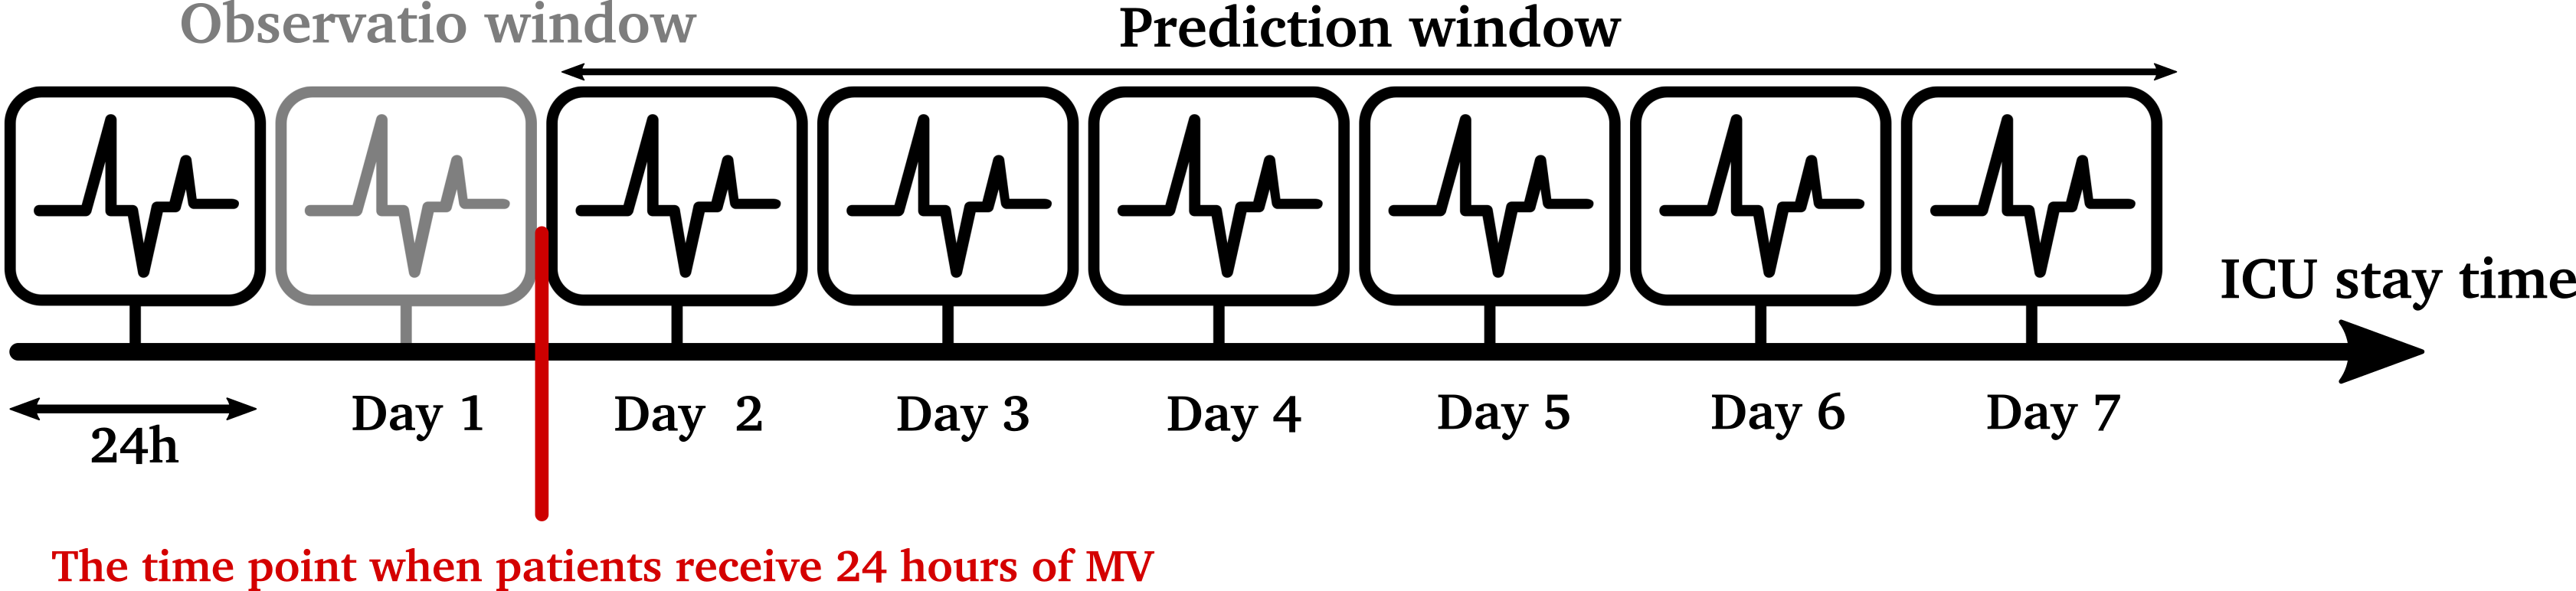
\includegraphics[width=0.9\linewidth]{images/windows.png}
    \caption{Observation and prediction windows in the MIMIC-IV dataset for predicting in-ICU mortality among mechanically ventilated patients.}
    \label{fig:windows}
\end{figure}

\subsubsection{ADNI dataset Description}
% Ravi please add info here
The Alzheimer's Disease Neuroimaging Initiative (ADNI) dataset (\href{https://adni.loni.usc.edu}{https://adni.loni.usc.edu}) is a longitudinal, multi-modal dataset designed to study the progression of Alzheimer's disease (AD) through various biomarkers. The dataset was launched in 2003 as a public-private partnership and has undergone multiple phases, including ADNI-1, ADNI-GO, ADNI-2, and ADNI-3, with the aim of improving early diagnosis and monitoring disease progression.

ADNI contains imaging data such as magnetic resonance imaging (MRI) and positron emission tomography (PET), as well as clinical assessments, cognitive test scores, and cerebrospinal fluid (CSF) biomarkers. The dataset includes individuals classified into three major groups: cognitively normal (CN) controls, individuals with mild cognitive impairment (MCI), and those diagnosed with Alzheimer's disease (AD). This rich multimodal data provides a comprehensive view of disease progression and enables machine learning models to identify potential biomarkers and patterns indicative of Alzheimer's pathology.

To preprocess the dataset, we standardized imaging-derived features, normalized biomarker values, and imputed missing data using mean feature values. The final dataset included 99 features. The target variable was the patient diagnosis being either Normal Cognitive function, mild cognitive impairment or Alzheimer's disease.

\subsection{General workflow}
In the following we will describe the general workflow of our graph-based approach, starting from the knowledge graph creation from scientific articles, through model training and SHAP-based optimization, up to interpreting ML predictions using the refined knowledge graph and SHAP values. Figure \ref{fig:workflow} shows a conceptual flow diagram of the original workflow idea. All the corresponding code can be found at \href{https://github.com/Prgrmmrjns/GRACE}{https://github.com/Prgrmmrjns/GRACE}. Our implementation supports multiple LLM providers, including OpenAI and Ollama, making the approach more accessible and adaptable to different computational environments. We leverage XGBoost, a gradient-boosting algorithm, for its performance and capabilities in handling structured data and interaction constraints. Model parameters and early stopping are configured for optimal performance. The dataset is separated into training, validation, and test sets, with the validation set used for hyperparameter optimization and early stopping during model training.

\begin{figure}
    \centering
    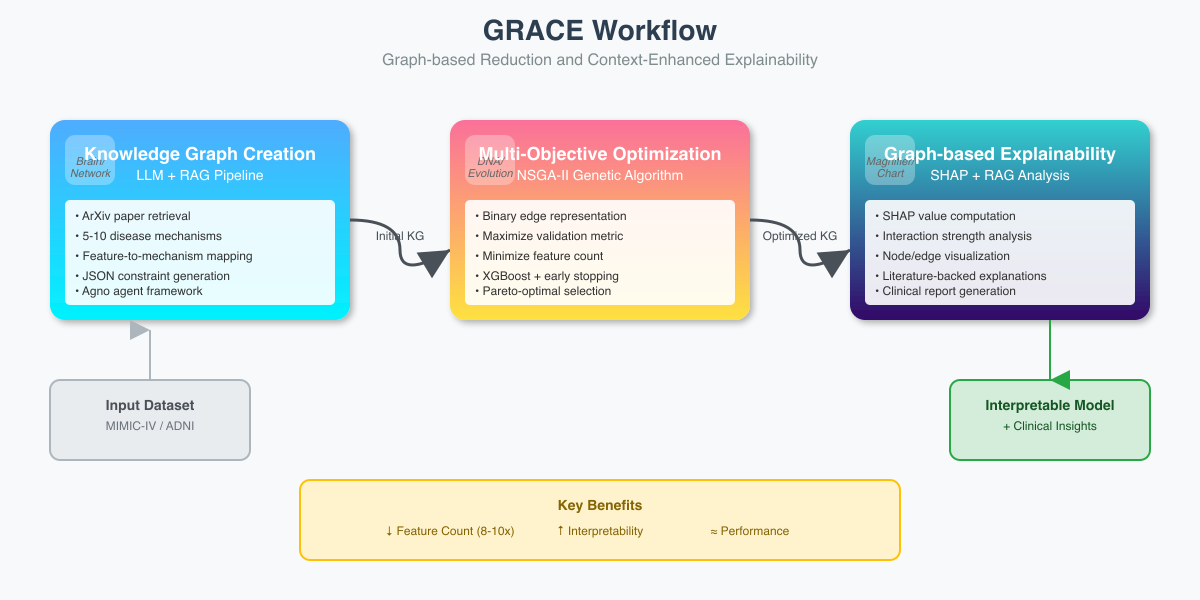
\includegraphics[width=\linewidth]{images/general_workflow.png}
    \caption{General workflow of GRACE. \textbf{A}: The LLM is asked to come up with disease mechanisms that link input features to target variable. The LLM is informed by dataset description and can retrieve information from scientific articles selected by keywords. The LLM then iterates through all disease mechanisms and assigns input nodes to each of them. The outcome is a knowledge graph consisting of input nodes representing dataset independent features (orange nodes), intermediate nodes of suggested disease mechanisms (blue nodes) and the target node representating the target variable (green node). \textbf{B}:  A separate model is trained for every intermediate node using input features connected to it. The node model predictions are fed to a meta-model to make the final predictions. During optimization we test which combinations of input features lead to the highest performance with the minimal amount of input features. \textbf{C}: LIME is used to interpret model predictions of an individual sample. This is done for each node model as well as the ensemble model. We also investigate LIME feature interactions.  \textbf{D}: The LLM aims to explain feature contributions and interactions by LIME based on scientific literature. The LLM will also give user-specific recommendations based on medical knowledge.}
    \label{fig:workflow}
\end{figure}

\subsubsection{Knowledge graph creation}
The first step of our workflow is the generation of a knowledge graph specific to the given dataset and prediction task and informed by provided dataset background information as well as additional database information such as domain knowledge specific ArXiv articles. 
As a prerequisite for the knowledge graph the user has to input a detailed description of the dataset and task at hand. Here the user should ideally outline what each dataset feature represents and how the features were processed. In addition the user has to specify the target column and provide keywords for the later RAG search.
Based on these user-customized information we leverage the \emph{agno} agent framework \href{https://docs.agno.com/introduction}{https://docs.agno.com/introduction} to build a task-specific knowledge graph through a Retrieval-Augmented Generation (RAG) loop. Scientific articles from ArXiv matching user-defined keywords are embedded and stored in a vector database (Lance DB). An agent then suggests 5-10 central disease mechanisms for the associated dataset and prediction task. In the corresponding prompt we input the user-provided dataset description, all dataset features including the target column. The LLM also has access to the provided knowledge bases provided by an ArXiv search from the user provided keywords. In the following step we then ask the LLM to subsequently assign dataset features to each of the earlier suggested disease mechanisms and again provide a dataset description and access to the knowledge base. After asking the LLM to assign features to any of the disease mechanisms we then check for any yet unassigned features and ask the LLM to assign them to any of the suggested groups. The KG creation is complete when all features are assigned to at least one of the disease mechanisms (see Figure \ref{fig:workflow}A for a created KG for the MIMIC dataset).

\subsubsection{Graph-based dimensionality reduction, prediction, and optimization}

\subsection{Evaluation setup}
We evaluated our knowledge graph-based dimensionality reduction approach across two distinct medical datasets with different characteristics and prediction goals. For performance assessment, we selected metrics aligned with each dataset's specific prediction task: area under the ROC curve (AUC) for the binary mortality prediction in MIMIC with unbalanced classes and multiclass accuracy for the three-class Alzheimer's diagnosis classification in ADNI.
We implemented 5-fold cross-validation with 30\% of data randomly assigned as the test set. For each fold we recreated the whole graph creation from scratch.
We benchmarked our approach against three established dimensionality reduction techniques, employing the same XGBoost ML model with the same parameters and early stopping mechanism. 
Next to performance we also compared the approaches in terms of features in the final ML model as well as run-time.

\subsection{Comparison setup}
\subsubsection{Baseline - no preprocessing}
Our baseline utilized the complete feature set without any dimensionality reduction, allowing XGBoost to perform implicit feature selection through its tree-based architecture. 

\subsubsection{PCA}
Principal Component Analysis transforms the feature space into orthogonal components that capture maximum variance. We implemented PCA with the number of components determined automatically to retain 95\% of the variance. While PCA efficiently reduces dimensionality through linear combinations of original features, its mathematical transformations lack clinical interpretation. The resulting principal components represent abstract mathematical constructs rather than domain-specific concepts, creating a fundamental trade-off between dimensionality reduction and interpretability.

\subsubsection{Recursive feature elimination}
Recursive Feature Elimination (RFE) provides a feature selection approach that iteratively removes the least important features based on model performance. Unlike our knowledge graph method, RFE selects individual features without organizing them into interpretable intermediate concepts, maintaining the original feature space without creating abstractions. 

\section{Results}

\subsection{Performance comparison}
% Table with results comparison

We conducted a comprehensive evaluation of our knowledge graph-based dimensionality reduction approach against established techniques to determine its effectiveness. Table \ref{tab:performance_comparison} presents the performance metrics across datasets, with several notable findings.

\begin{table}[h]
\centering
\begin{tabular}{l|cc|c|cc|c}
\hline
& \multicolumn{3}{c|}{ADNI (Accuracy)} & \multicolumn{3}{c}{MIMIC (AUC)} \\
Method & Mean & Std & Avg. Features & Mean & Std & Avg. Features \\
\hline
No Processing & 0.9433 & 0.0098 & 99.0 & 0.8122 & 0.0070 & 67.0 \\
PCA & 0.7932 & 0.0132 & 49.0 & 0.7683 & 0.0147 & 33.0 \\
RFE & 0.9433 & 0.0081 & 20.0 & 0.8035 & 0.0094 & 20.0 \\
GRACE & 0.9475 & 0.0147 & 10.0 & 0.7981 & 0.0118 & 18.4 \\
\hline
\end{tabular}
\caption{Comparison of dimensionality reduction techniques - Performance metrics and feature counts}
\label{tab:performance_comparison}
\end{table}

For the ADNI dataset, our knowledge graph-based approach (GRACE) achieved a classification accuracy of 0.9475, slightly outperforming the no-preprocessing baseline (0.9433) and Recursive Feature Elimination (RFE) (0.9433). While the performance gain is modest, GRACE achieved this result using only 10 features on average—a drastic reduction from the 99 features used by the baseline and the 20 features selected by RFE. The poor performance of Principal Component Analysis (PCA) (0.7932) highlights the limitations of purely statistical dimensionality reduction when applied to medical data with complex interrelationships.

For the MIMIC dataset, a different pattern emerged. The baseline approach with no preprocessing achieved the highest AUC (0.8122), closely followed by RFE (0.8035). Our GRACE approach (0.7981) performed competitively, ranking just below these methods but substantially better than PCA (0.7683). This performance differential likely stems from the more complex, heterogeneous nature of ICU data in MIMIC compared to the more structured neurological assessments in ADNI.

A key finding across both datasets is the trade-off between predictive performance and model complexity. For MIMIC, while GRACE did not achieve the highest AUC, it delivered a strong score using the fewest features (18.4) compared to the baseline (67) and RFE (20). This dramatic dimensionality reduction creates more interpretable models without a substantial loss in performance, demonstrating a compelling balance between accuracy and explainability—a critical factor in medical applications where understanding feature relationships is often as important as raw predictive power.

\subsection{Knowledge graph structures}
The knowledge graphs generated by our framework serve as the backbone for both dimensionality reduction and enhanced interpretability. The process begins with an LLM-based agent that analyzes the dataset features and relevant scientific literature to propose a set of underlying biological or clinical mechanisms. These mechanisms act as intermediate nodes, grouping related features together.

For the ADNI dataset, the agent identified eight central mechanisms representing key pathophysiological processes in Alzheimer's disease. Figure \ref{fig:adni_graphs} illustrates this transformation from the initial, comprehensive knowledge graph to the optimized, sparse structure. The following analysis represents one example run of our system.

\textbf{Initial Knowledge Graph Structure:} The agent's initial analysis of the ADNI dataset resulted in eight distinct mechanisms: "Amyloid Pathology" (30 features), "Tauopathy" (51 features), "Neurodegeneration" (51 features), "Metabolic" (34 features), "Cognitive" (63 features), "Neuropsychiatric" (35 features), "Risk Factors" (29 features), and "Modifiers" (31 features). The initial graph contained 109 nodes and 367 edges, with an average of 3.7 edges per feature, reflecting the complex interconnections between biomarkers across different pathological processes.

The agent's reasoning demonstrates sophisticated domain-knowledge integration, identifying mechanisms such as "Amyloid-beta Pathology and Plaque Deposition" which encompasses the accumulation of amyloid-beta peptides leading to extracellular amyloid plaques. This mechanism appropriately groups cerebrospinal fluid biomarkers (ABETA42, ABETA40), PET imaging tracers (PIB, AV45, FBB), and related neurodegeneration markers, reflecting the agent's understanding of the underlying pathophysiology.

\textbf{Optimized Knowledge Graph Structure:} The optimization process dramatically reduced the graph complexity while preserving predictive performance. In this example run, the optimization converged to 3 final constraint groups containing 13 total features (down from 99), with the graph structure containing only 22 nodes and 253 edges. The optimization identified three key merged mechanisms:

\begin{enumerate}
\item \textbf{Group 1} (2 features): A focused biomarker cluster
\item \textbf{Group 2} (4 features): Core cognitive assessment measures  
\item \textbf{Group 3} (7 features): Integrated pathological indicators
\end{enumerate}

The optimized graph demonstrates how the algorithm identifies the most informative feature combinations while maintaining interpretable groupings. Each remaining feature in the optimized graph represents multiple original mechanisms, as evidenced by the complex labels in the GraphML structure where individual nodes carry labels such as "Amyloid, Cognitive, Functional/Subjective, Metabolic, Neurodegenerative, Neuropsychiatric, Risk Factors, Tau/Neurodegenerative, Vascular/Cardiometabolic", indicating their multi-mechanism significance.

\begin{figure}[h!]
    \centering
    \begin{subfigure}[b]{\textwidth}
        \centering
        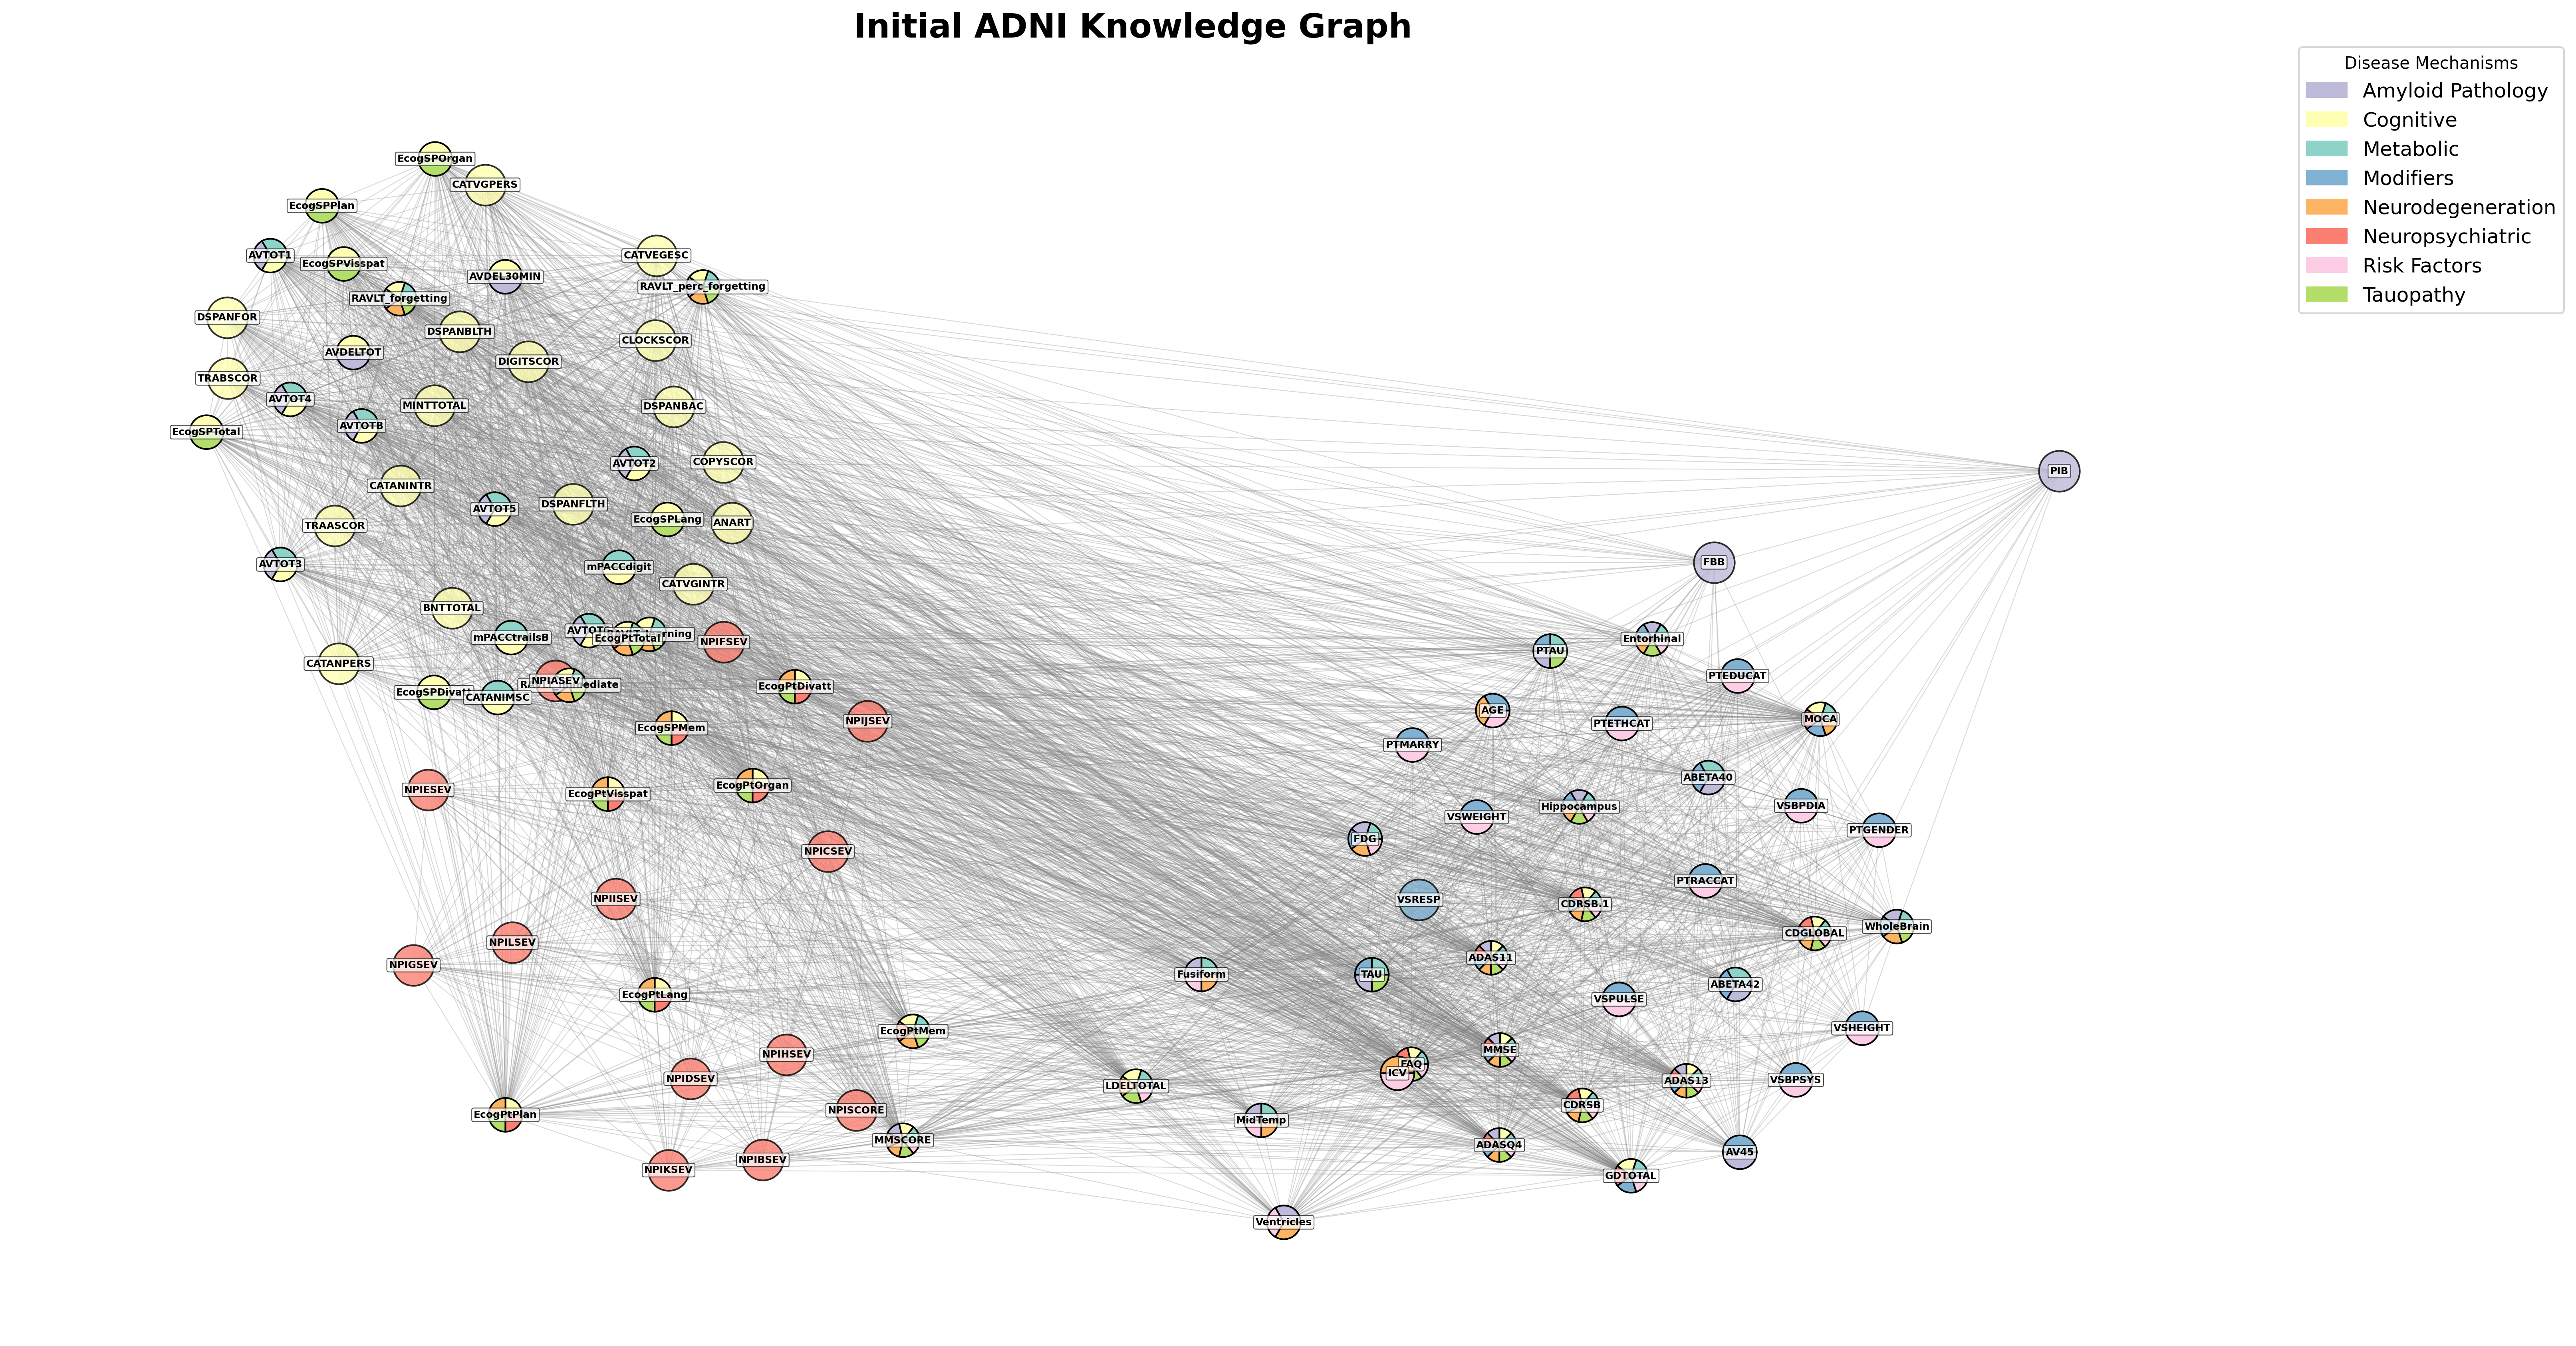
\includegraphics[width=\textwidth]{images/adni_initial_kg.png}
        \caption{Initial ADNI Knowledge Graph showing 8 distinct disease mechanisms identified by the LLM agent, with 99 features organized into biologically meaningful groups.}
        \label{fig:adni_initial_kg}
    \end{subfigure}
    
    \vspace{1cm}
    
    \begin{subfigure}[b]{\textwidth}
        \centering
        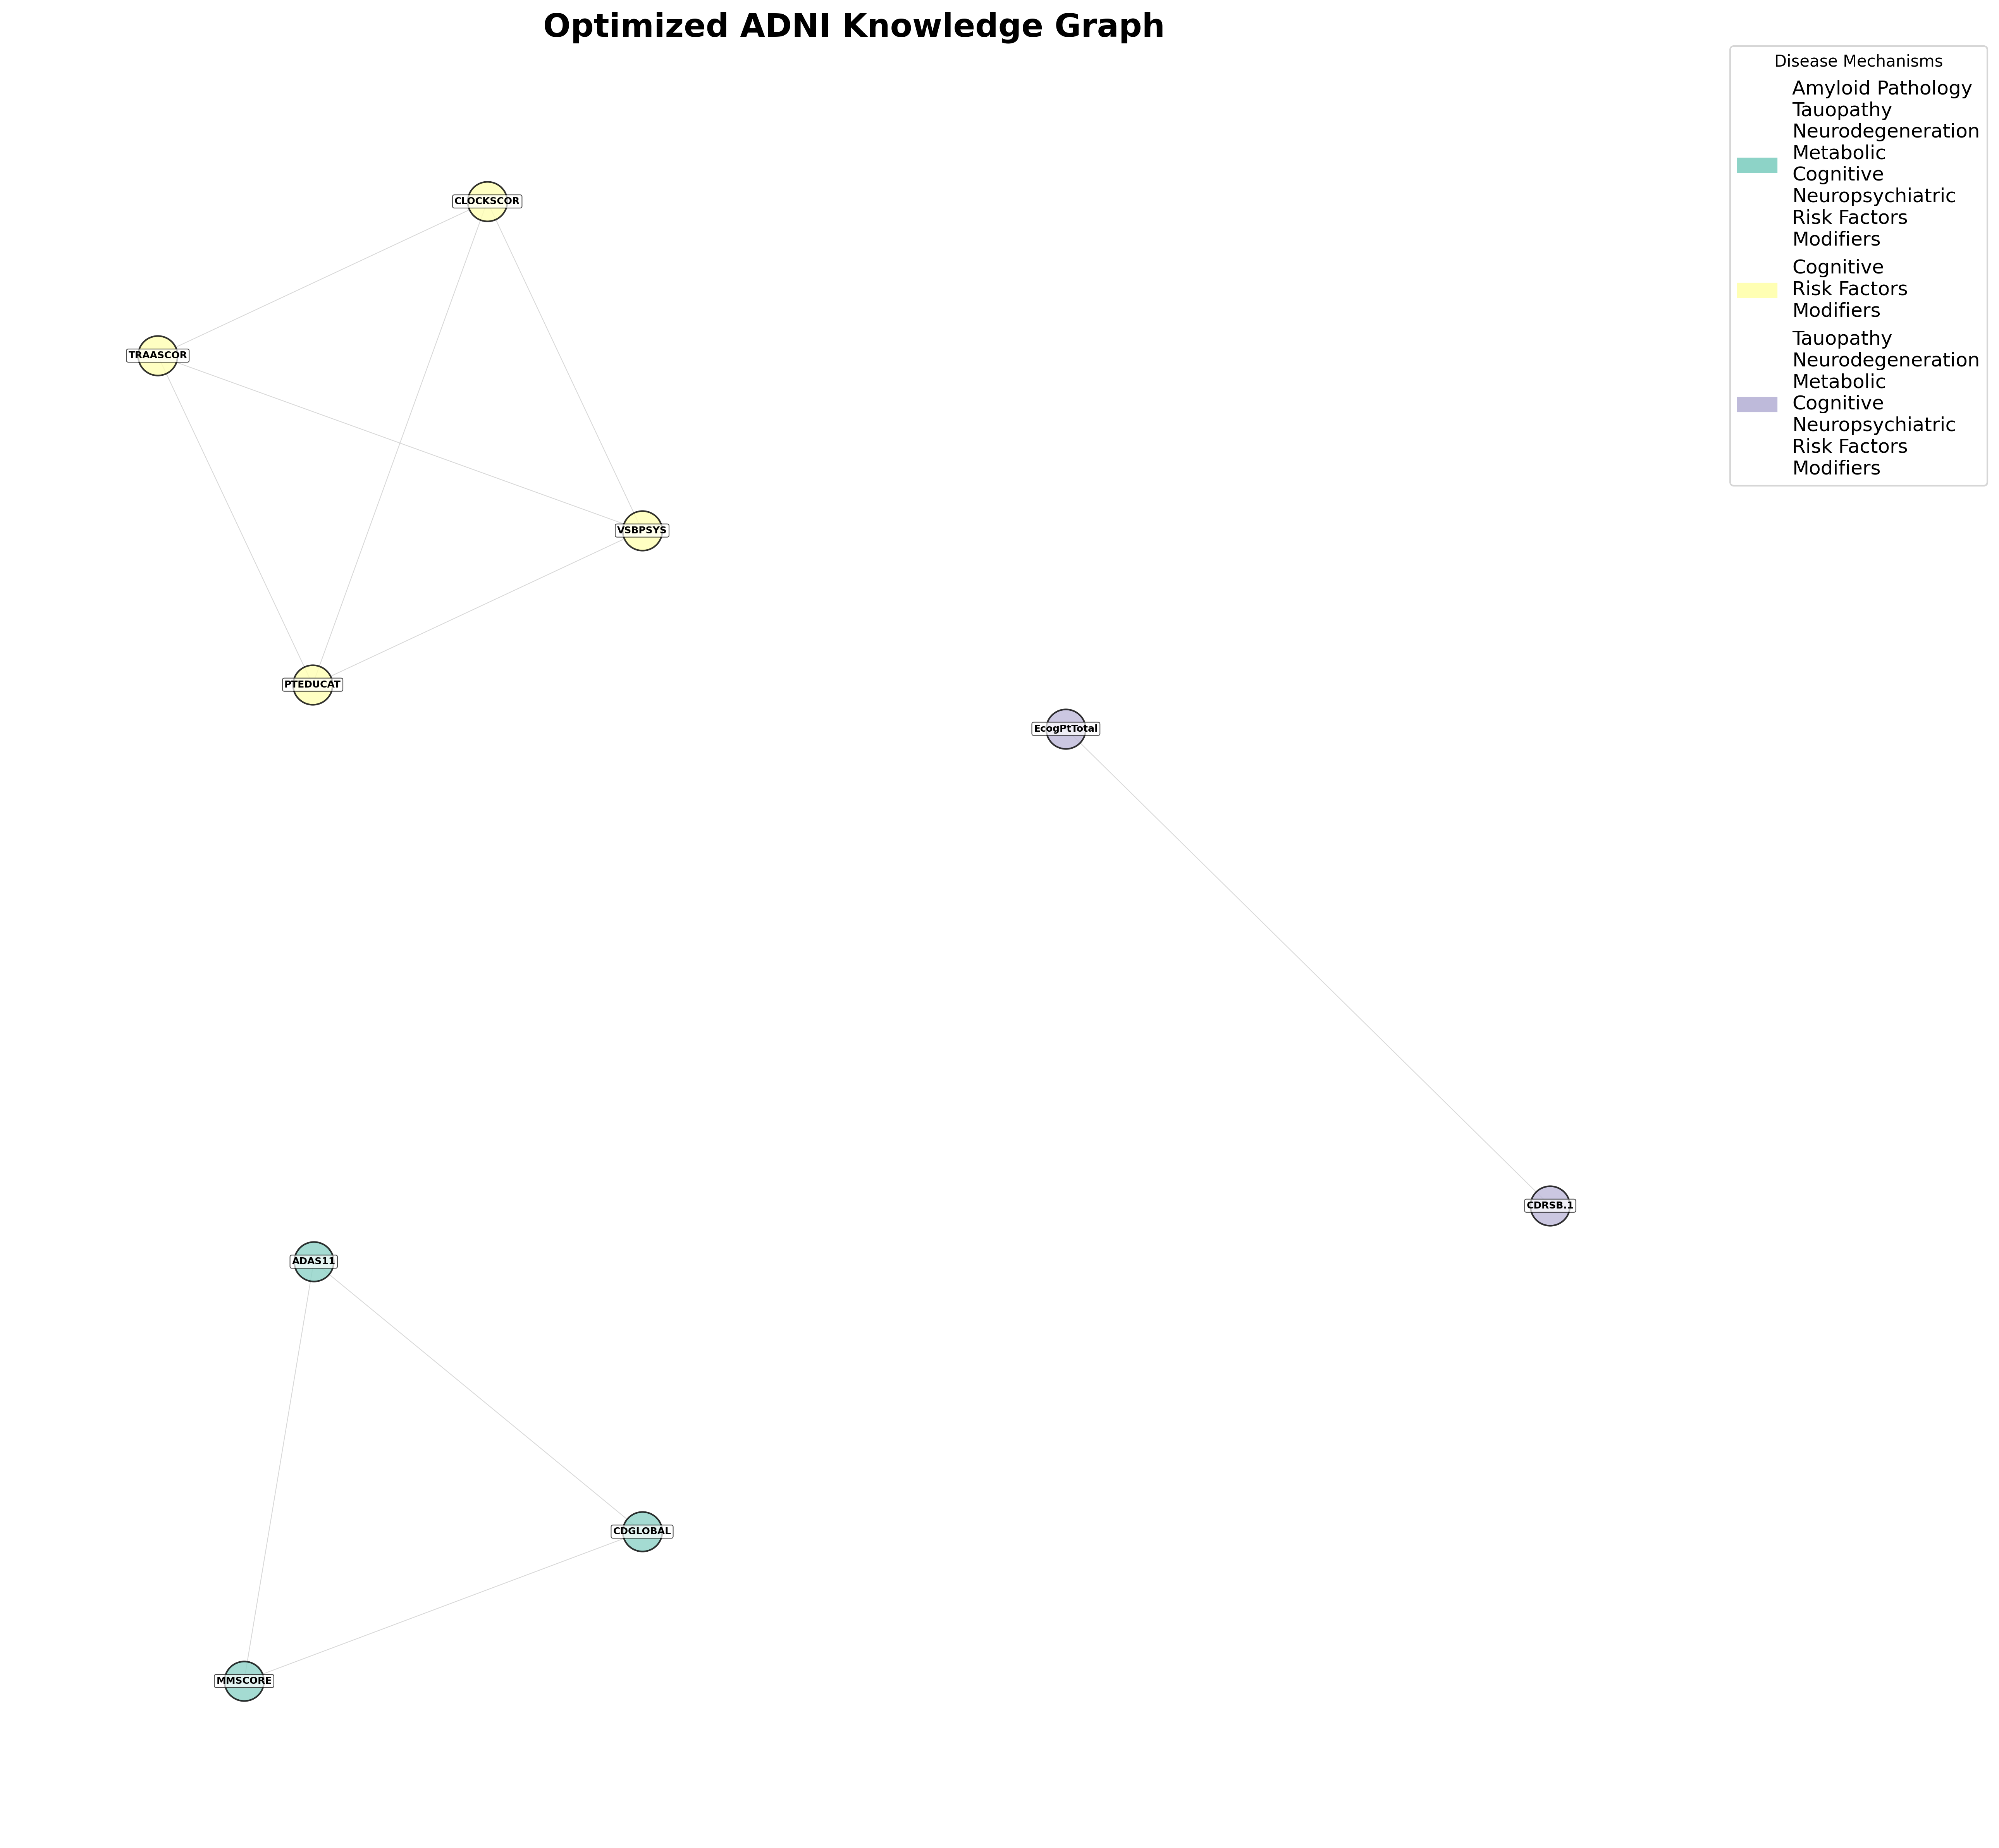
\includegraphics[width=\textwidth]{images/adni_optimized_kg.png}
        \caption{Optimized ADNI Knowledge Graph after multi-objective optimization, reduced to 13 features organized into 3 constraint groups while maintaining predictive performance.}
        \label{fig:adni_optimized_kg}
    \end{subfigure}
    \caption{Knowledge graph evolution for the ADNI dataset (example from a single run). The optimization process achieves an 87\% reduction in features while preserving the interpretable structure through merged mechanism labels that reflect the biological significance of retained features.}
    \label{fig:adni_graphs}
\end{figure}

This optimization represents a compelling balance between model complexity and biological interpretability. The retained features span multiple original mechanisms, suggesting that the most predictive biomarkers are those that capture information across several pathological processes simultaneously. It is important to note that these results represent a single example run, and the specific graph structures and optimization outcomes may vary across different executions due to the stochastic nature of both the LLM agent and the optimization algorithm.

\subsection{Interpretability using knowledge graph - Case study}
To demonstrate the clinical interpretability advantages of our knowledge graph approach, we conducted detailed SHAP (SHapley Additive exPlanations) analyses on the optimized models for both datasets. This analysis reveals how individual features and their interactions contribute to predictions while maintaining the biological context provided by the knowledge graph structure, enhanced by AI-powered clinical interpretations grounded in scientific literature.

\subsubsection{GRACE for Alzheimer's Disease Prediction}

Figure \ref{fig:shap_analysis_adni} presents the SHAP-weighted knowledge graph for the ADNI dataset, where node colors represent disease mechanisms and edge characteristics show feature importance and interactions. The radial layout with the target variable at the center enables clear visualization of how each biomarker contributes to Alzheimer's diagnosis predictions.

\begin{figure}[h!]
    \centering
    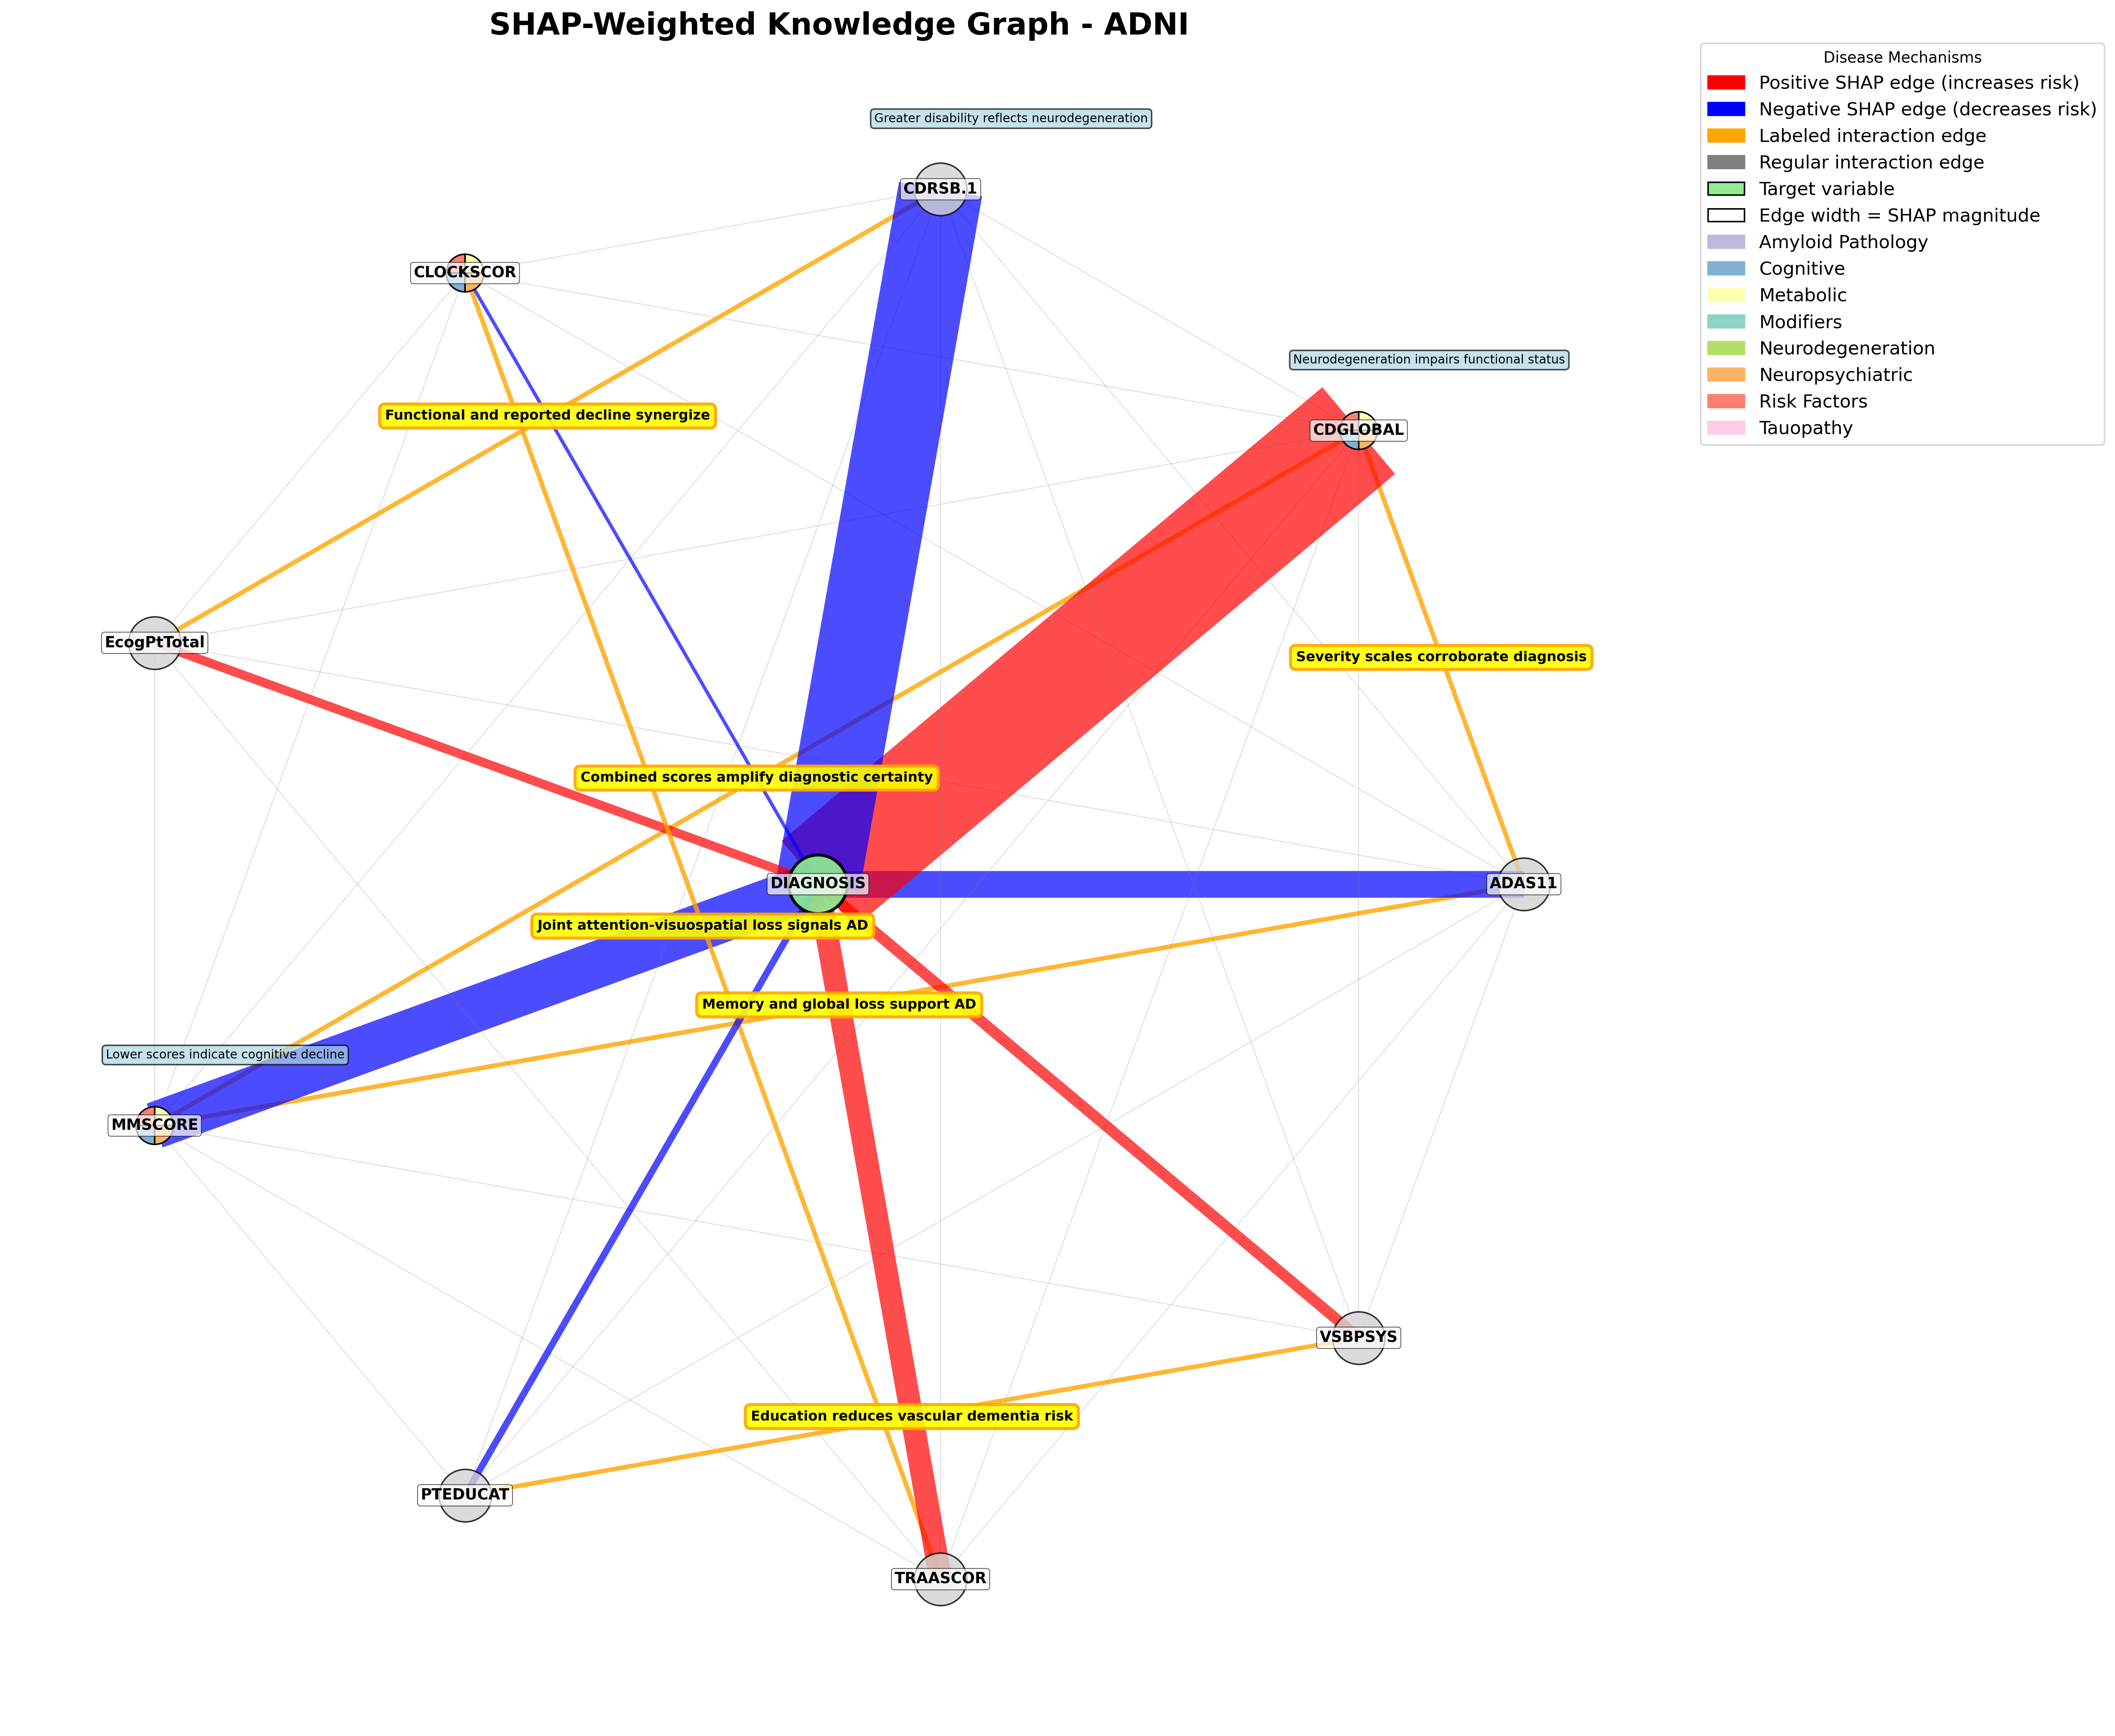
\includegraphics[width=\textwidth]{images/adni_shap_interpreted_graph.png}
    \caption{SHAP-weighted knowledge graph for ADNI dataset showing Alzheimer's disease prediction. The target diagnosis is at the center, with biomarkers arranged radially. Red edges indicate features that increase Alzheimer's risk, blue edges show protective factors, and orange highlighted edges represent significant feature interactions with AI-generated causal explanations. Node colors reflect disease mechanisms (amyloid pathology, neurodegeneration, etc.), while edge thickness corresponds to feature importance magnitude.}
    \label{fig:shap_analysis_adni}
\end{figure}

\subsubsection{GRACE for ICU Mortality Prediction}

Figure \ref{fig:shap_analysis_mimic} demonstrates the application of GRACE to critical care medicine using the MIMIC dataset for ICU mortality prediction. The knowledge graph organizes clinical variables by physiological systems, with AI-generated explanations providing insights into the underlying pathophysiological mechanisms driving mortality risk.

\begin{figure}[h!]
    \centering
    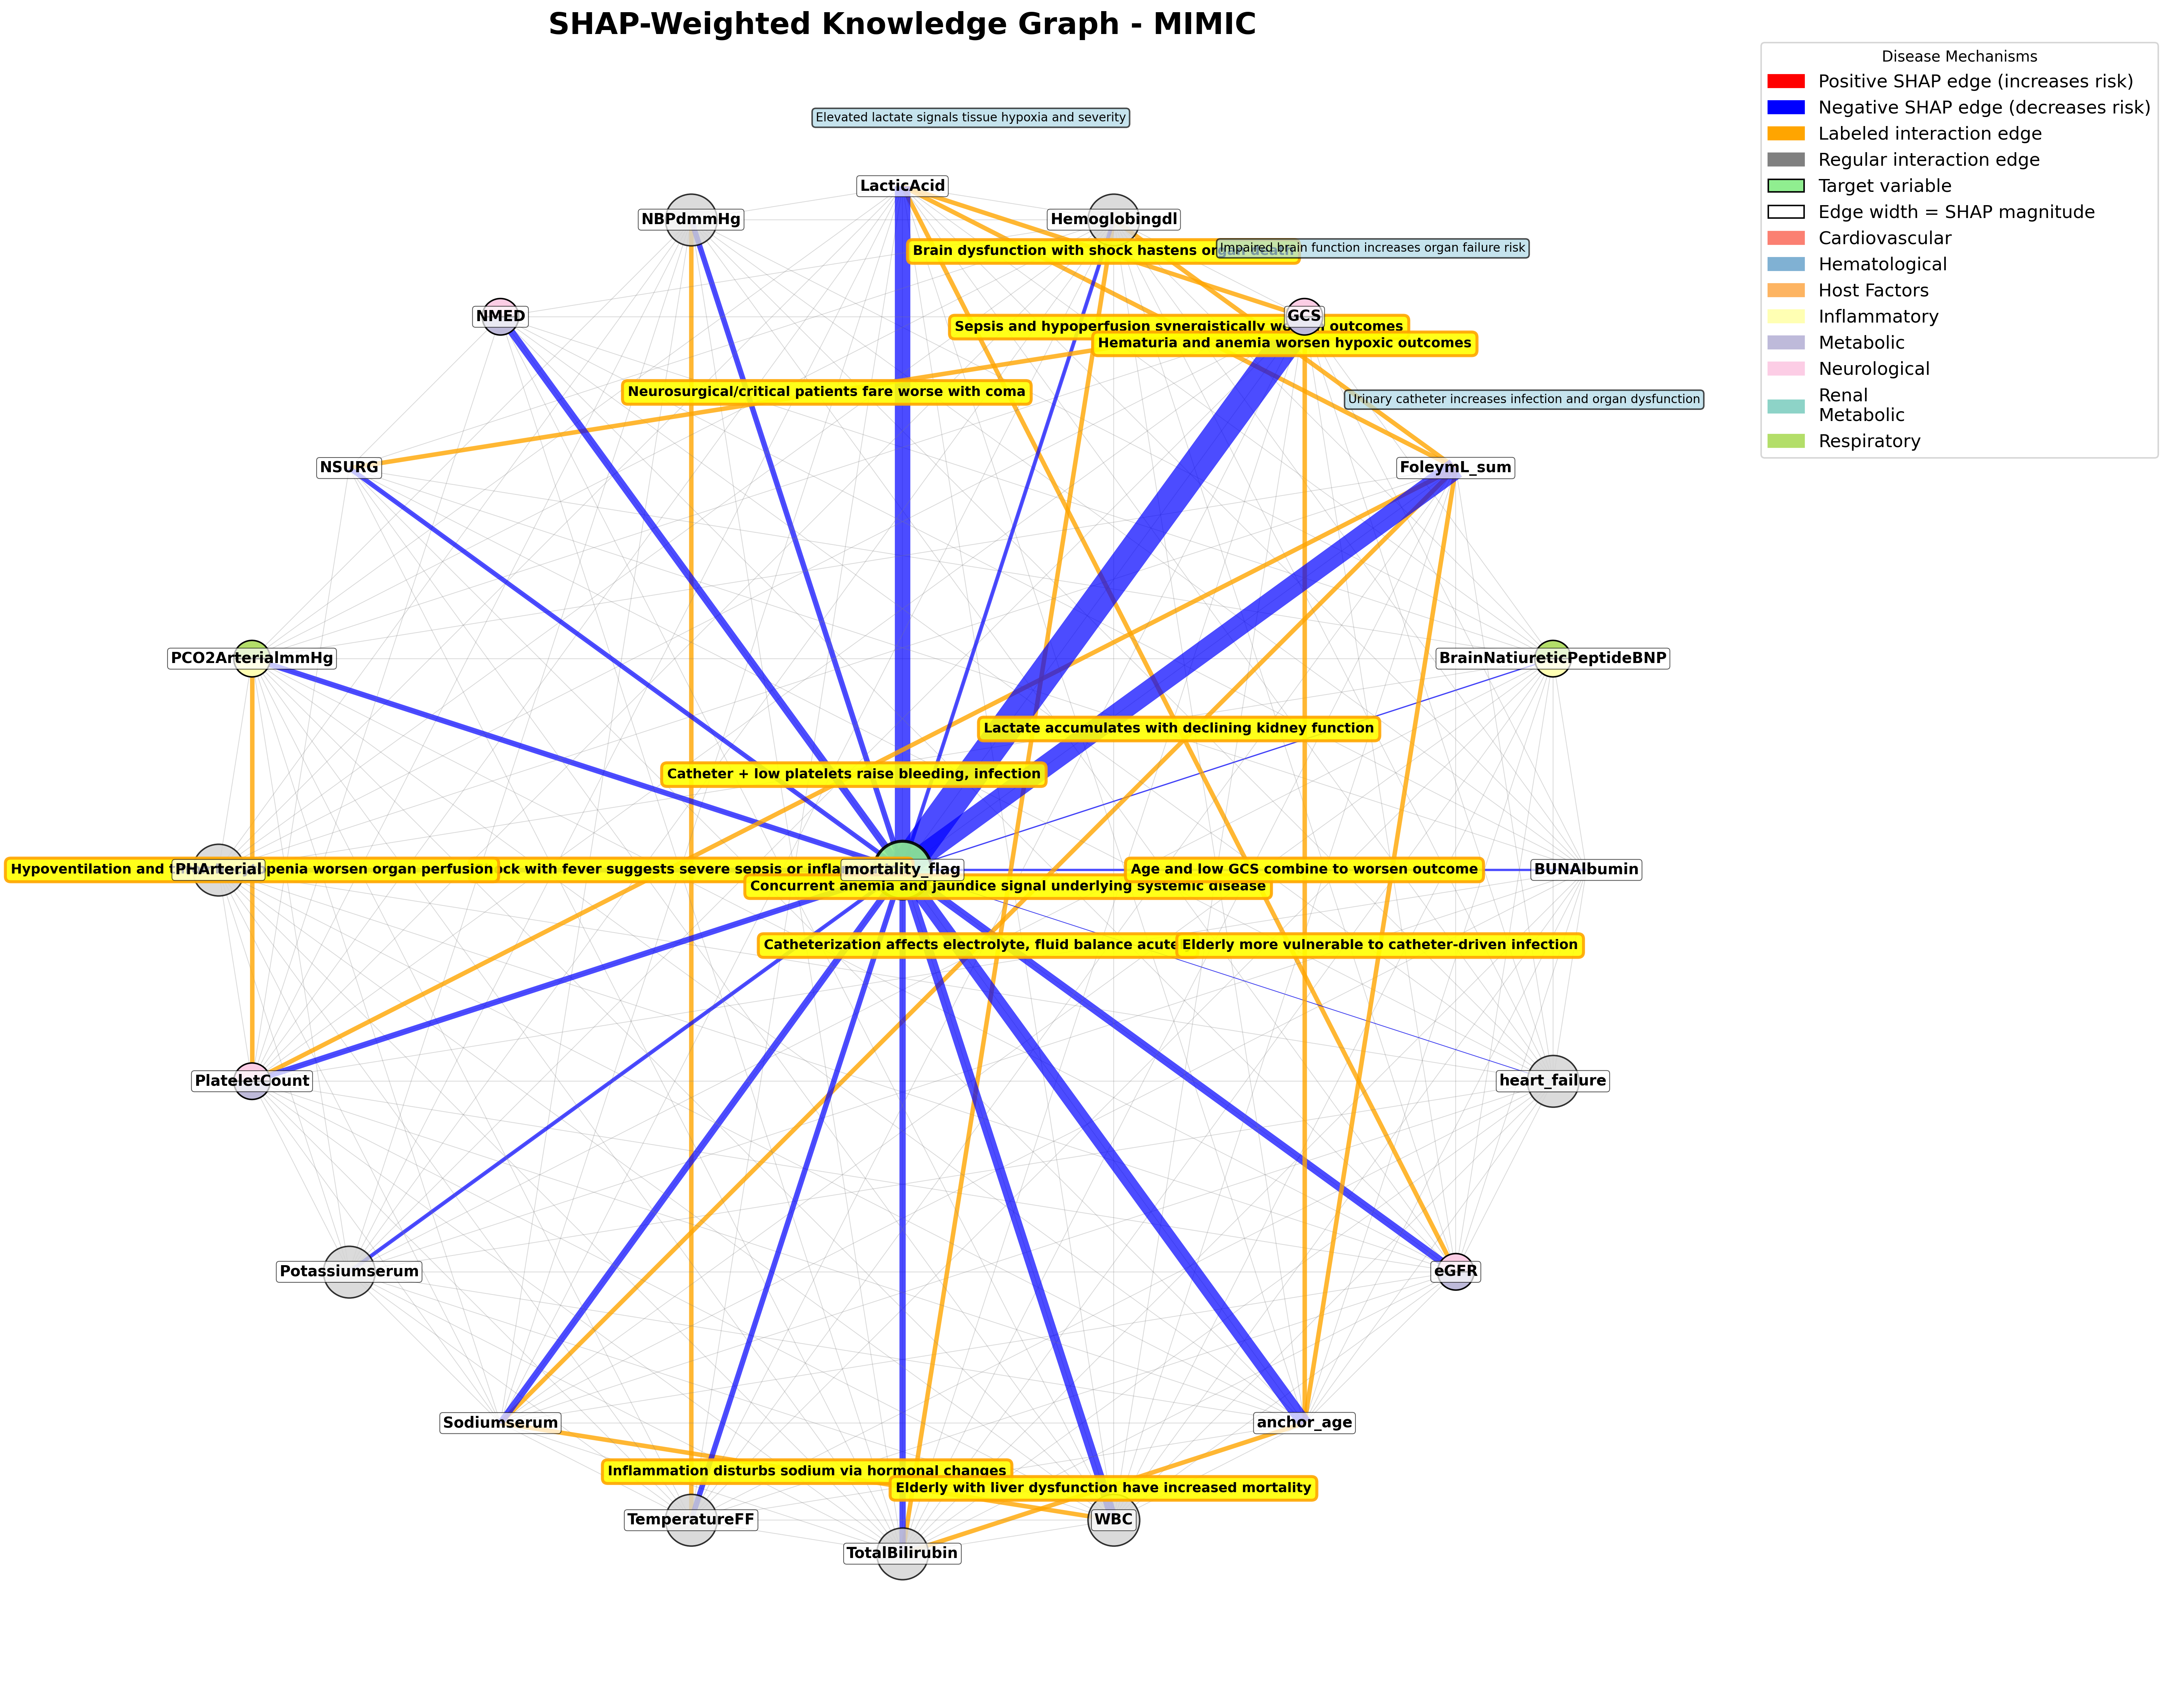
\includegraphics[width=\textwidth]{images/mimic_shap_interpreted_graph.png}
    \caption{SHAP-weighted knowledge graph for MIMIC dataset showing ICU mortality prediction. Clinical variables are organized by physiological systems (circulatory, respiratory, metabolic, etc.) around the central mortality target. Red edges indicate factors that increase mortality risk, blue edges show protective factors. Orange highlighted edges with causal explanations reveal critical feature interactions such as organ failure cascades and multi-system dysfunction patterns that drive ICU outcomes.}
    \label{fig:shap_analysis_mimic}
\end{figure}

\subsubsection{Clinical Decision Support Through AI-Enhanced Interpretability}

The GRACE framework provides several key advantages for clinical interpretation:

\begin{enumerate}
    \item \textbf{Causal Understanding}: Unlike traditional feature importance methods, GRACE combines SHAP values with AI-generated explanations that describe the underlying biological mechanisms. For example, rather than simply showing that creatinine is important, the system explains "kidney damage reduces filtration" as the causal mechanism.
    
    \item \textbf{Domain Knowledge Integration}: The knowledge graph structure preserves clinically meaningful relationships between features, organizing them by disease mechanisms (e.g., inflammatory, metabolic, neurological) rather than statistical correlations alone.
    
    \item \textbf{Literature-Grounded Interpretations}: Through Retrieval-Augmented Generation (RAG), the AI agent grounds its explanations in current scientific literature, providing evidence-based rationales for feature interactions and contributions.
    
    \item \textbf{Multi-System Perspective}: The framework reveals how features from different physiological systems interact to influence outcomes, particularly important in complex conditions like multi-organ failure or neurodegenerative disease.
\end{enumerate}

\textbf{Example Clinical Insights:} In the MIMIC mortality prediction model, GRACE identified critical interactions between respiratory and circulatory parameters, explaining how "reduced oxygen delivery causes organ failure" - a clinically relevant insight that helps physicians understand the cascade of events leading to mortality. Similarly, in ADNI, the system revealed how "neuronal death from protein aggregation" links amyloid and tau pathology to cognitive decline.

The comprehensive clinical interpretations generated by our AI agent provide detailed explanations for each feature and interaction, grounded in current medical literature. These interpretations include biological pathways, causal mechanisms, and actionable insights for practitioners. The complete interpretation reports, containing detailed analyses of all features and interactions, are available in the supplementary materials\footnote{Complete SHAP interpretation reports with detailed clinical explanations: \texttt{adni\_shap\_interpretation\_report.json} and \texttt{mimic\_shap\_interpretation\_report.json}}.

\subsubsection{Clinical Workflow Integration}

This interpretability approach addresses a critical gap in clinical machine learning deployment. While traditional ML models provide predictions, GRACE provides \textit{understanding} - explaining not just what the model predicts, but why, grounded in established medical knowledge. This enables:

\begin{itemize}
    \item \textbf{Clinical Validation}: Physicians can verify that model decisions align with known pathophysiology
    \item \textbf{Educational Value}: The system can teach medical students and residents about disease mechanisms
    \item \textbf{Hypothesis Generation}: Novel feature interactions identified by the model can suggest new research directions
    \item \textbf{Trust and Adoption}: Explainable predictions increase clinician confidence in AI-assisted decision making
\end{itemize}

The result is an interpretable machine learning system that not only achieves high predictive performance but also provides clinically meaningful insights that can guide medical decision-making, support clinical education, and accelerate biomedical research through AI-enhanced understanding of complex disease processes.

\section{Discussion}


\bibliographystyle{unsrt}
\bibliography{references}

\end{document}
